%要运行该模板,LaTex需要安装CJK库以支持汉字.

%字体大小为12像素,文档类型为article

%如果你要写论文,就用report代替article

%所有LaTex文档开头必须使用这句话

\documentclass[12pt]{article}

%这两行是用于段落首行缩进
\usepackage{indentfirst}
\setlength{\parindent}{2em}

%使用支持汉字的CJK包

\usepackage{ctex}


%开始CJK环境,只有在这句话之后,你才能使用汉字

%另外,如果在Linux下,请将文件的编码格式设置成GBK

%否则会显示乱码

\usepackage{lipsum}

%用listings展示Python代码
\usepackage{listings}
\usepackage{color}

\definecolor{dkgreen}{rgb}{0,0.6,0}
\definecolor{gray}{rgb}{0.5,0.5,0.5}
\definecolor{mauve}{rgb}{0.58,0,0.82}

\lstset{frame=tb,
	language=Python,
	aboveskip=3mm,
	belowskip=3mm,
	showstringspaces=false,
	columns=flexible,
	basicstyle={\small\ttfamily},
	numbers=none,
	numberstyle=\tiny\color{gray},
	keywordstyle=\color{blue},
	commentstyle=\color{dkgreen},
	stringstyle=\color{mauve},
	breaklines=true,
	breakatwhitespace=true,
	tabsize=3
}

	
	%这是文章的标题
	
	\title{Deep News Nankai}
	
	%这是文章的作者
	
	\author{李兴贺 1611071}
	
	%这是文章的时间
	
	%如果没有这行将显示当前时间
	
	%如果不想显示时间则使用 \date{}
	
	\date{2018/12/14}
	
	%以上部分叫做"导言区",下面才开始写正文
	
	\begin{document}
		
		%先插入标题
		
		\pagenumbering{gobble}
		
		\maketitle
		
		\newpage
		
		%再插入目录
		
		\tableofcontents
		
		\newpage
		
		\pagenumbering{arabic}
		
		\section{Deep News搜索引擎简介}
		
		这学期选了温老师的信息检索系统原理,第三次作业是要做一个Deep Web Search Engine。说实话,直到完成这次的代码编写和测试工作,我仍然对这个Deep的真正含义不是很清楚。
		
		虽然不是很清楚,但是我不能就这么坐以待毙呀,想起温老师曾经说过,这次作业和普通的搜索引擎相比,就是爬虫的部分写法不太一样,我深以为然,开始一步一步动手做出这个项目。
		
		
		
		%第二段使用黑体,上面的一个空行表示另起一段
		
		%\CJKfamily{hei}LaTex 将空格和制表符视为相同的距离.
		
		\begin{figure}[htb]
			\centering
			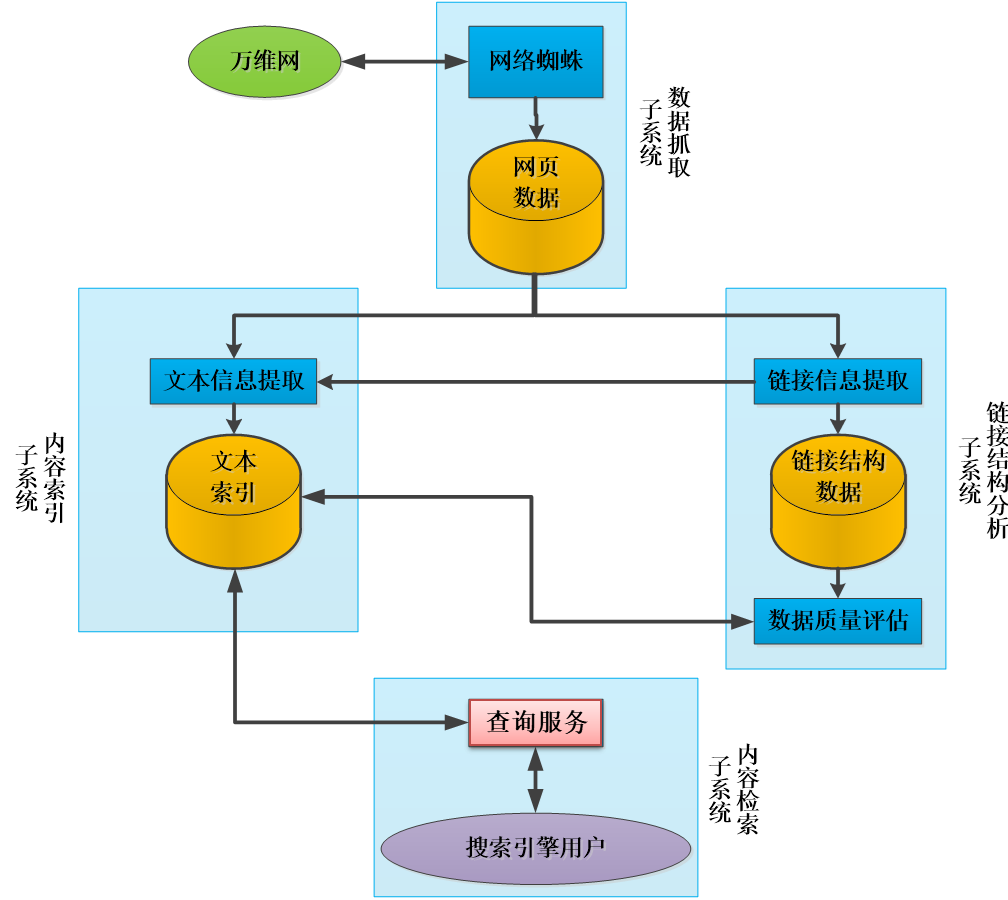
\includegraphics[width=0.5\linewidth]{screenshot001}
			\caption[搜索引擎体系结构]{搜索引擎体系结构}
			\label{搜索引擎体系结构}
		\end{figure}
		
		通常,搜索引擎体系结构由四个部分构成,分别是数据抓取子系统、内容索引子系统、链接结构分析子系统、内容检索子系统。
		Deep News也不例外,下面我将演示搜索引擎的使用,并分别介绍这几个子系统的设计、实现和调用。
		
		\newpage
		
		\section{系统环境}
		
		系统:Windows10
		
		编程语言: Python3.6
		
		Python模块: math operator datetime configparser time os xml 
		
		sqlite3(数据库)
		
		jieba(中文分词)
		 
		flask(web框架)
		  
		requests(HTTP库) 
		
		newspaper(新闻处理)
		
		pyinstaller(py打包exe)
		
		~\\
		
		本项目已将内容检索子系统打包成exe文件,可以在没有Python环境的系统下直接运行。其他子系统均需要以上Python模块,可以运行../deep-news/env.py一键安装环境。
		
		本项目中唯一的配置文件是../deep-news/config.ini,配置文件的解析由configparser模块完成。
		
		\newpage
		
		\section{Deep News使用说明}
		
		运行../deep-news/main.exe(其实是快捷方式,本体是../deep-news/web/main.exe)
		
		\begin{figure}[htb]
			\centering
			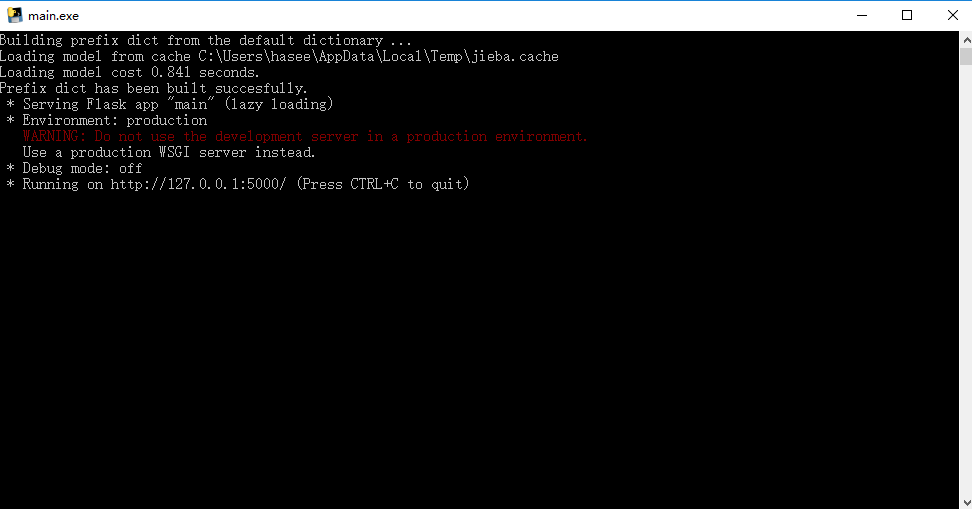
\includegraphics[width=0.7\linewidth]{screenshot002}
			\caption[main.exe后台运行截图]{main.exe后台运行截图}
			\label{main.exe后台运行截图}
		\end{figure}
		
		按照命令行提示,接下来打开浏览器,输入127.0.0.1:5000 进入搜索引擎主界面。
		
		\begin{figure}[htb]
			\centering
			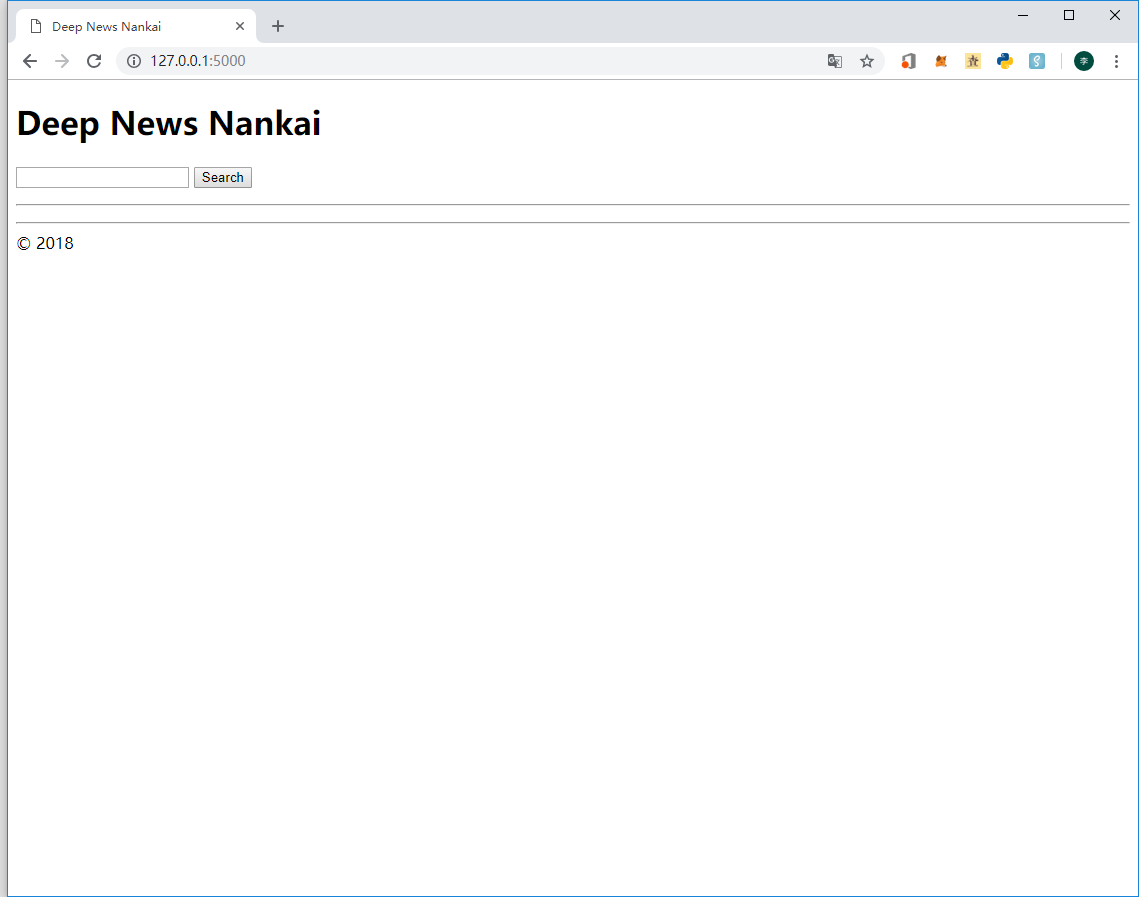
\includegraphics[width=0.6\linewidth]{screenshot003}
			\caption[Deep News 初始界面]{Deep News 初始界面}
			\label{Deep News 初始界面}
		\end{figure}
		
		\newpage
		
		在搜索栏输入想要搜索的内容,点击"Search"进行检索。Deep-News提供三种检索方式,可以在搜索栏下方点击"相关度"、"时间"或"热度",再点击"Ok",修改检索方式。
		
		\begin{figure}[htb]
			\centering
			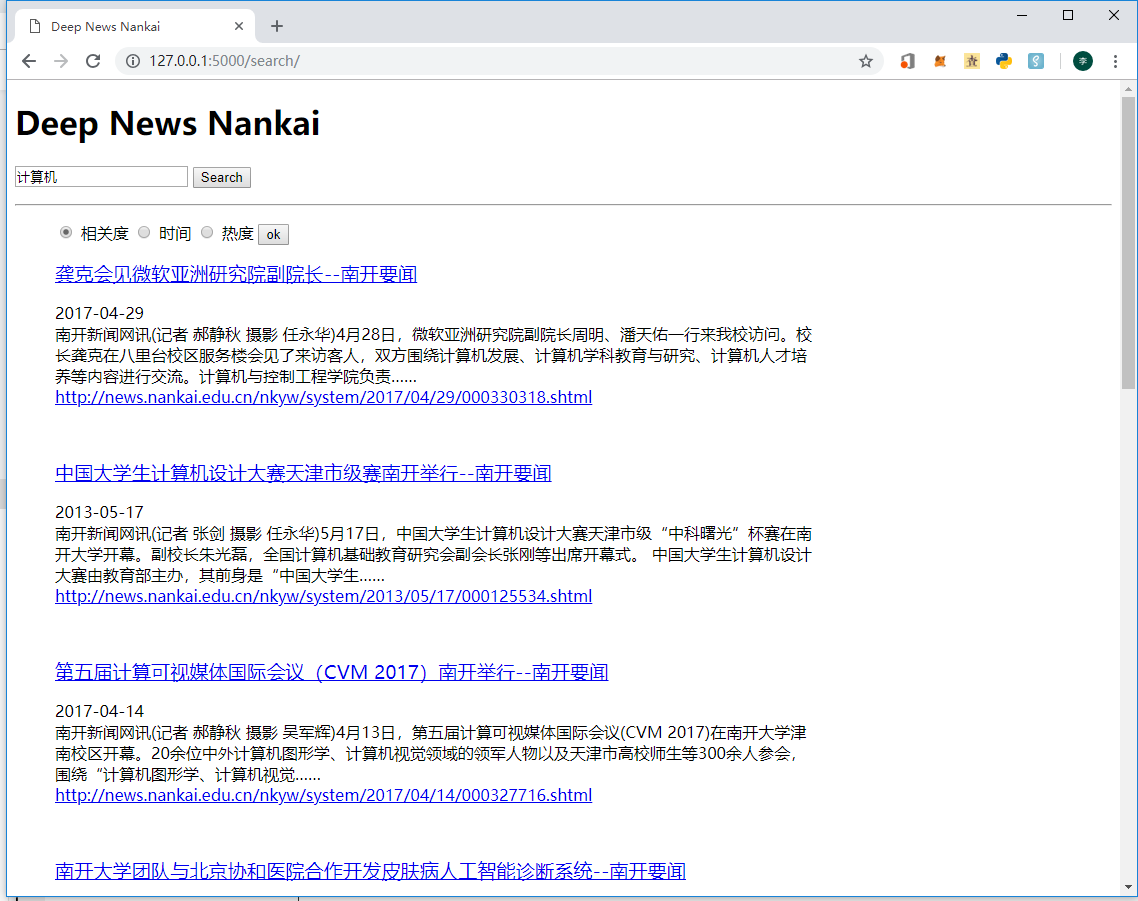
\includegraphics[width=0.8\linewidth]{screenshot004}
			\caption[检索页面示例1]{检索页面示例1}
			\label{检索页面示例1}
		\end{figure}
		
		\newpage
		
		页面底部可以自由跳页查看全部检索结果。
		
		\begin{figure}[htb]
			\centering
			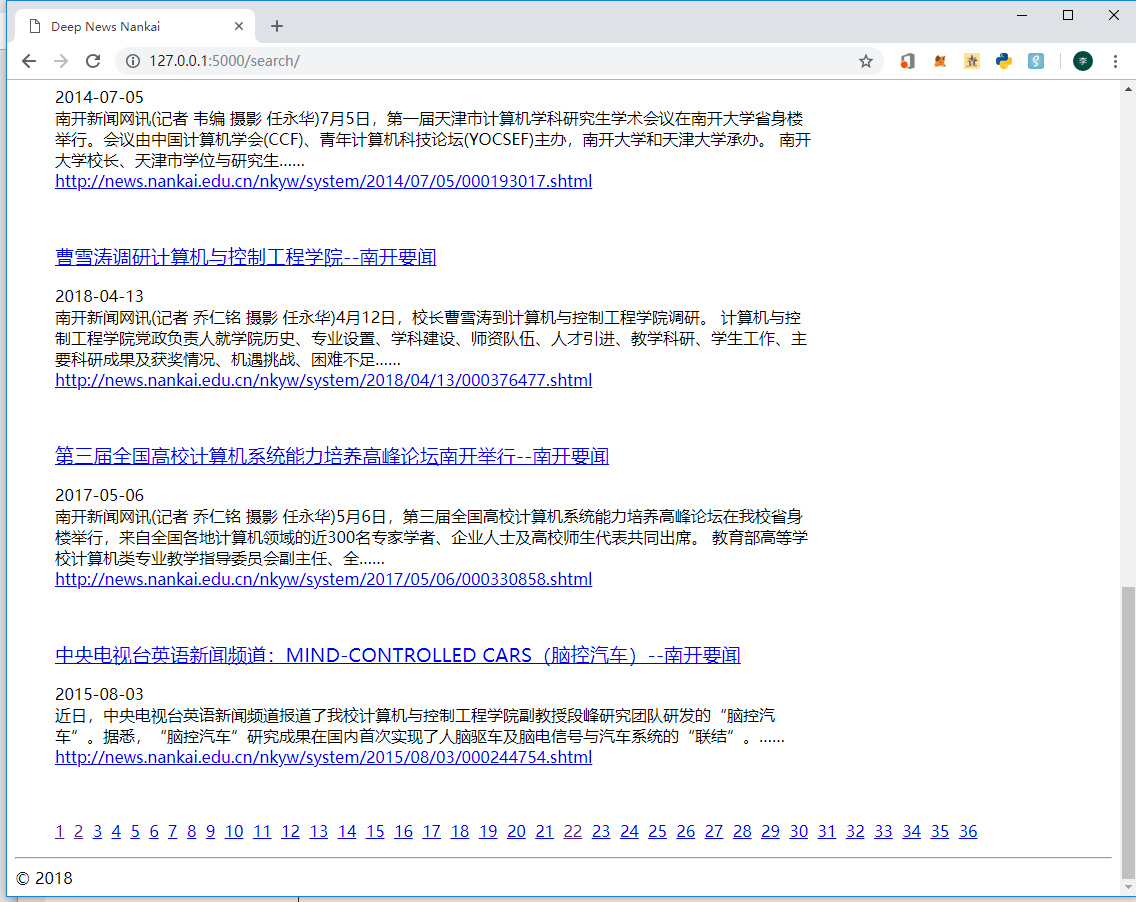
\includegraphics[width=0.5\linewidth]{screenshot005}
			\caption[检索页面示例2]{检索页面示例2}
			\label{检索页面示例2}
		\end{figure}
		
		\begin{figure}[htb]
			\centering
			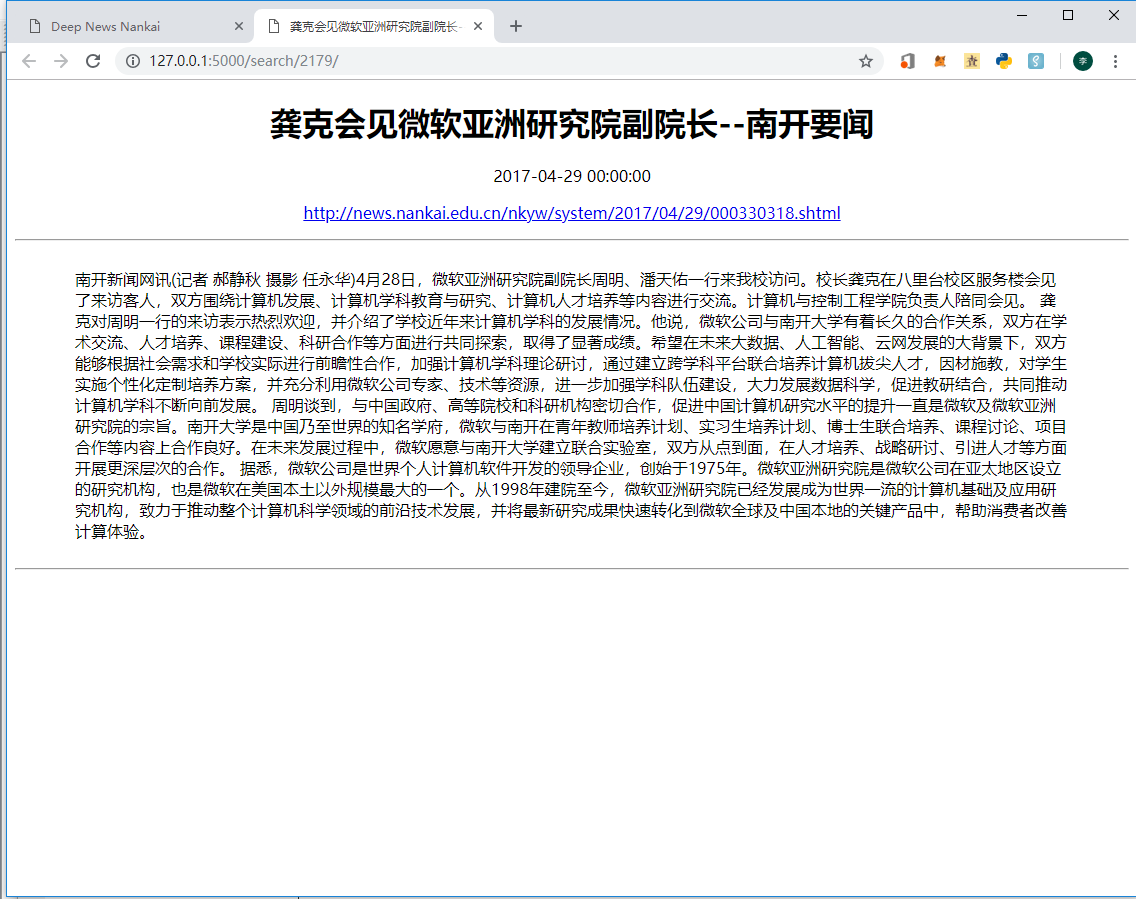
\includegraphics[width=0.5\linewidth]{screenshot006}
			\caption[检索结果示例]{检索结果示例}
			\label{检索结果示例}
		\end{figure}
	
		\newpage
		
		\begin{figure}[htb]
			\centering
			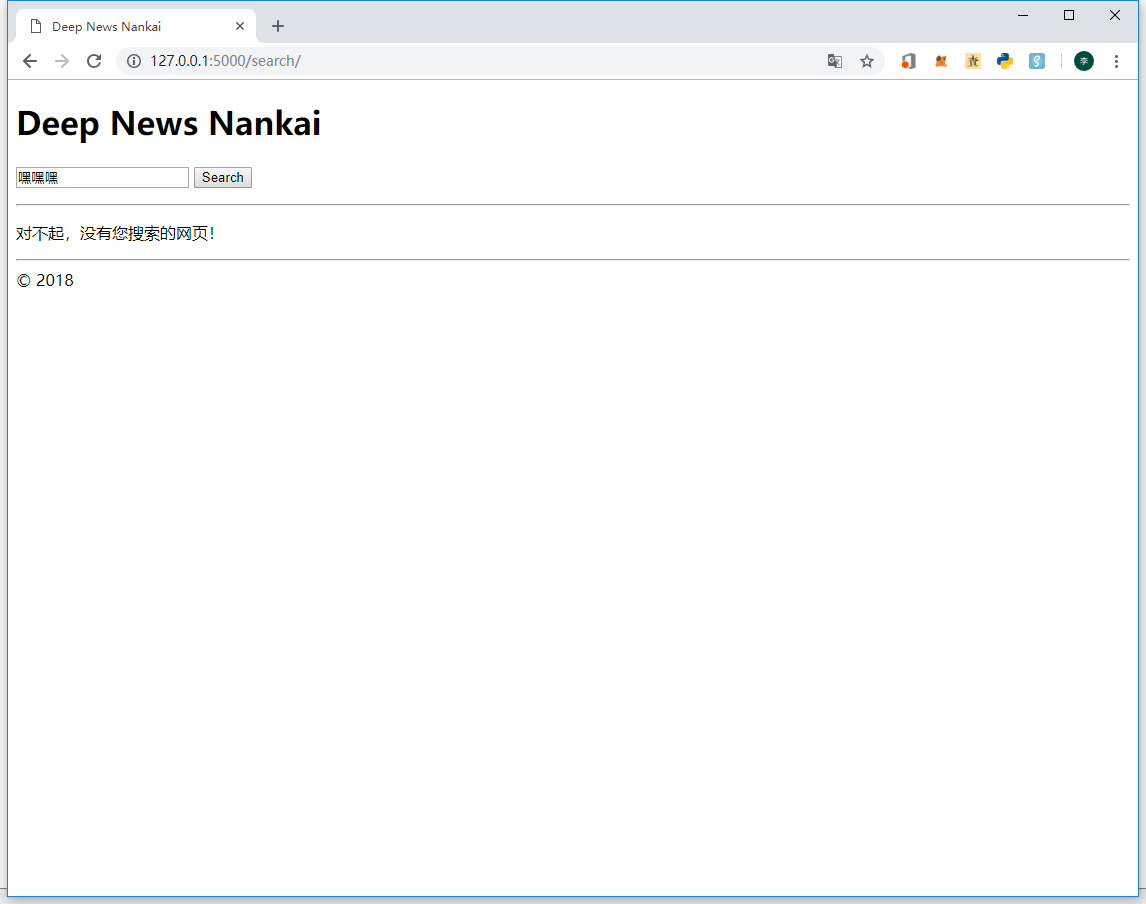
\includegraphics[width=0.7\linewidth]{screenshot007}
			\caption[检索失败示例]{检索失败示例}
			\label{检索失败示例}
		\end{figure}
		
		
		\newpage
		
		\section{数据抓取子系统}
		
		源码 ../deep-news/code/spider.py
		
		抓取目标:南开大学新闻网(http://news.nankai.edu.cn/)
		
		抓取页面数量:11143
		
		这里选择南开大学新闻网的原因是,网页的html代码相对比较规整(其实是用现有的工具可以解析),并且爬虫运行过程中并不需要登录也不用面对验证码。
		数据抓取子系统的思路是遍历整个网站,将新闻内容的链接加入newspool,然后访问newspool中的每个链接向其发送get请求并对返回的页面进行解析,
		将得到的有效信息保存在../data/news/xxx.xml文件中。(事实上,得到了一万多个xml文件后,我们甚至可以不做一个搜索引擎,转而做一个“南开大学旧闻网”。
		显然,这并没有什么意义)。newspool中所有的链接都爬取过后,数据抓取子系统的工作就结束了。
		
		
		\begin{lstlisting}
		def get_news_pool():
			news_pool = []
			for i in range(200,243):
				temp=442-i
				target = 'http://news.nankai.edu.cn/nkyw/system/more/32000000/0002/32000000_00000'+str(temp)+'.shtml'
				req = requests.get(url = target)
				html = req.text
				bf = BeautifulSoup(html)
				texts = bf.find_all('a', class_ = 'news')
				for i in range(len(texts)):
					url=str(texts[i])
					start=url.find('http')
					end=url.find('shtml')+5
					url=url[start:end]
					news_pool.append(url)
				time.sleep(t)				
		return(news_pool)
		\end{lstlisting}
		
		这是get-news-pool函数的部分代码,工作流程为循环遍历http://news.nankai.edu.cn/nkyw/system/more/下的每一个页面,
		向其发送get请求,将返回的html页面用beautisoup处理后得到每条新闻的url,将url加入news-pool,
		工作完成后函数返回的是列表news-pool
		
		~\\
		
		\begin{lstlisting}
		def crawl_news(news_pool,min_body_len,doc_dir_path,doc_encoding):
			i=1
			for news in news_pool:
				article=Article(news,language='zh')
				try:
					article.download()
					article.parse()
				except Exception as e:
					print("-----%s: %s-----"%(type(e), news))
					continue
				doc=ET.Element("doc")
				ET.SubElement(doc, "id").text = "%d"%(i)
				ET.SubElement(doc, "url").text = news
				ET.SubElement(doc, "title").text = article.title
				ET.SubElement(doc, "datetime").text = str(article.publish_date)
				ET.SubElement(doc, "body").text = article.text
				tree = ET.ElementTree(doc)
				tree.write(doc_dir_path + "%d.xml"%(i), encoding = doc_encoding, xml_declaration = True)
				i += 1
		\end{lstlisting}
		
		crawl-news主要使用的是newspaper模块,提取出news-pool中每个url指向的新闻链接的标题、正文、时间,并连同url一起存进xml文件中。
		其中,Article是newspaper模块用来存储文章的对象,article.download()和article.parse()分别对该article对象进行下载和解析。
		实际爬取过程中可能出现异常,我们将异常情况输出至控制台并跳过该url继续执行下一条。
		
		\newpage
		
		\section{内容索引子系统}
		
		源码 ../deep-news/code/index.py
		
		内容索引子系统是搜索引擎中至关重要的部分。index.py主要实现了一个index module类,构建索引的所有操作都是该类的成员函数。
		
		\begin{lstlisting}
		class IndexModule:
			stop_words = set()
			postings_lists = {}
			
			config_path = ''
			config_encoding = ''
		\end{lstlisting}
		
		IndexModule类的成员变量。分别是停用词、记录列表、配置文件路径、编码。
		
		\begin{lstlisting}
		def construct_postings_lists(self):
			config = configparser.ConfigParser()
			config.read(self.config_path, self.config_encoding)
			files = listdir(config['DEFAULT']['doc_dir_path'])
			AVG_L = 0
			for i in files:
				try:
					root = ET.parse(config['DEFAULT']['doc_dir_path'] + i).getroot()
					title = root.find('title').text
					body = root.find('body').text
					docid = int(root.find('id').text)
					date_time = root.find('datetime').text
					seg_list = jieba.lcut(title + '。' + body, cut_all=False)
					
					ld, cleaned_dict = self.clean_list(seg_list)
					
					AVG_L = AVG_L + ld
					
					for key, value in cleaned_dict.items():
						d = Doc(docid, date_time, value, ld)
						if key in self.postings_lists:
							self.postings_lists[key][0] = self.postings_lists[key][0] + 1 # df++
							self.postings_lists[key][1].append(d)
						else:
							self.postings_lists[key] = [1, [d]] # [df, [Doc]]
				except Exception as e:
					print("-----%s: %s-----"%(type(e), i))
					continue
			AVG_L = AVG_L / len(files)
			config.set('DEFAULT', 'N', str(len(files)))
			config.set('DEFAULT', 'avg_l', str(AVG_L))
			with open(self.config_path, 'w', encoding = self.config_encoding) as configfile:
				config.write(configfile)
			self.write_postings_to_db(config['DEFAULT']['db_path'])
		\end{lstlisting}
		
		倒排索引构建算法使用内存式单遍扫描索引构建方法(SPIMI),其实就是依次对每篇新闻进行分词,
		如果出现新的词项则插入到词典中,否则将该文档的信息追加到词项对应的倒排记录表中。
		
		使用了jieba中文分词系统,效果还是很不错的,不用太操心。停用词列表是从别的搜索引擎项目中直接拿来的,应用中没有发现什么问题。
		
		倒排索引构建完成后将其写入数据库中。	
		
		\begin{lstlisting}
		def write_postings_to_db(self, db_path):
			conn = sqlite3.connect(db_path)
			c = conn.cursor()
			
			c.execute('''DROP TABLE IF EXISTS postings''')
			c.execute('''CREATE TABLE postings
			(term TEXT PRIMARY KEY, df INTEGER, docs TEXT)''')
			
			for key, value in self.postings_lists.items():
				doc_list = '\n'.join(map(str,value[1]))
				t = (key, value[0], doc_list)
			c.execute("INSERT INTO postings VALUES (?, ?, ?)", t)
			
			conn.commit()
			conn.close()
		\end{lstlisting}
		
		数据库采用的是sqlite3,写入的记录格式下图所示。
		
		\begin{figure}[h]
			\centering
			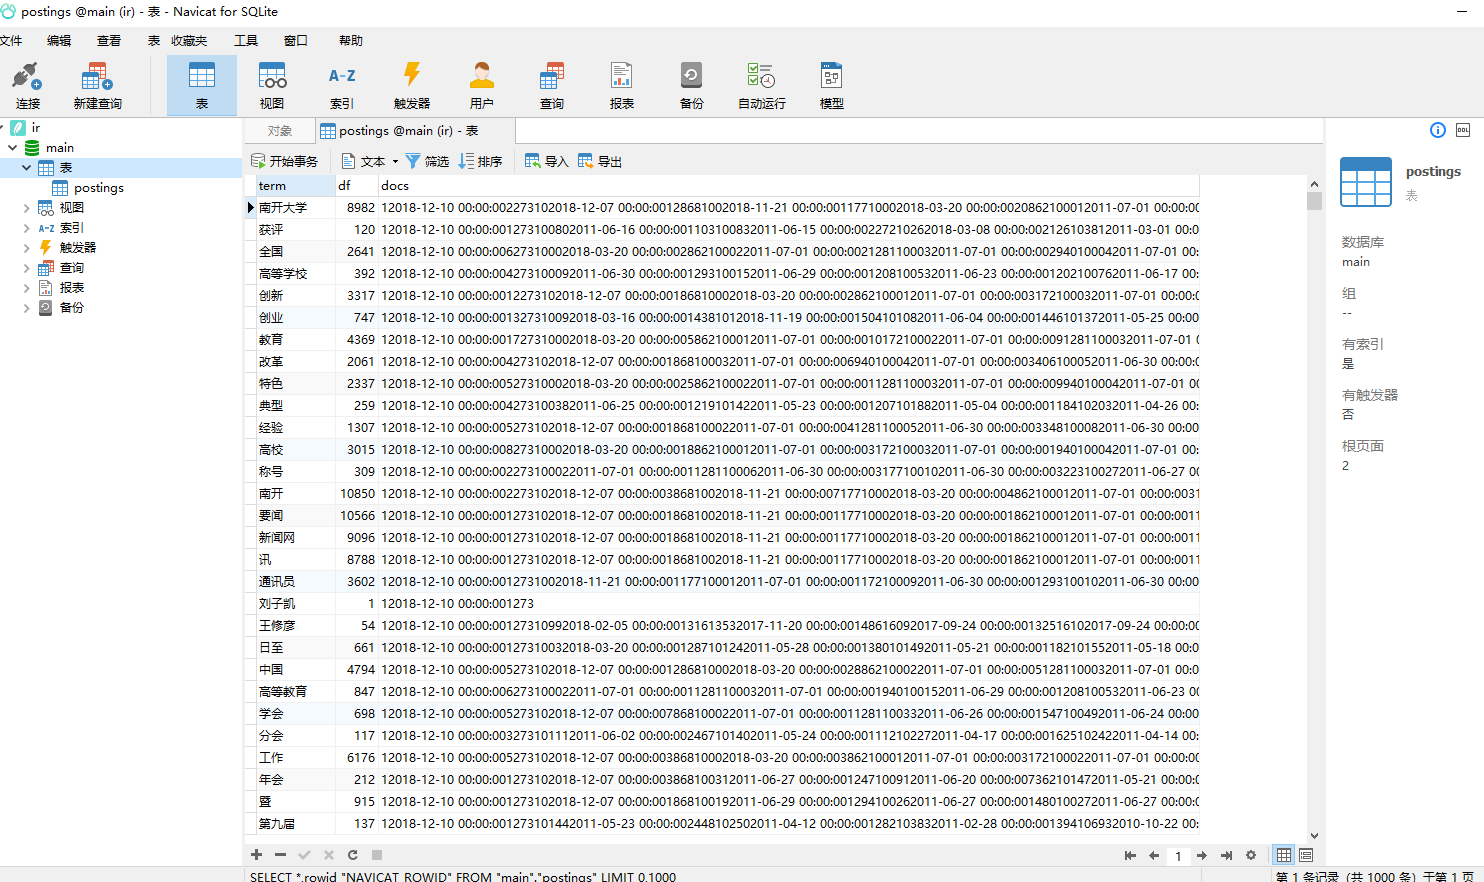
\includegraphics[width=0.7\linewidth]{screenshot008}
			\caption[倒排记录表可视化]{倒排记录表可视化}
			\label{倒排记录表可视化}
		\end{figure}
		
		
		\newpage
		
		\section{链接结构分析子系统}
		
		进行到这一步的时候,我发现了严重的问题。南开大学新闻网并没有推荐系统。
		
		以http://news.nankai.edu.cn/nkyw/system/2018/12/15/000423674.shtml这篇新闻为例,网页中不包含其他新闻的链接,
		导致PageRank无从做起。但是我曾经选过大数据计算及应用的课程,课程的大作业是实现PageRank算法......
		所以我只能将那次大作业一并上传,以示友好。PageRank在../deep-news/source/Pagerank目录下。
		
		\newpage
		
		\section{内容检索子系统}
		
		源码 ../deep-news/web/search engine.py
		
		Deep News支持三种检索类型,分别是相关度检索、时间倒序检索、热度检索。其中相关度检索采用经典的tf-idf算法,
		时间倒序是按新闻发布时间倒序排列,热度采用的是时间/相关度混合算法。
		
		\begin{lstlisting}
		def result_by_tfidf(self, sentence):
			seg_list = jieba.lcut(sentence, cut_all=False)
			n, cleaned_dict = self.clean_list(seg_list)
			TFIDF_scores = {}
			for term in cleaned_dict.keys():
				r = self.fetch_from_db(term)
				if r is None:
				continue
				df = r[1]
				docs = r[2].split('\n')
				for doc in docs:
					docid, date_time, tf, ld = doc.split('\t')
					docid = int(docid)
					tf = int(tf)
					ld = int(ld)
					tf=tf/ld
					idf=math.log2(self.N/df)
					s = tf*idf
					if docid in TFIDF_scores:
						TFIDF_scores[docid] = TFIDF_scores[docid] + s
					else:
						TFIDF_scores[docid] = s
				TFIDF_scores = sorted(TFIDF_scores.items(), key = operator.itemgetter(1))
				TFIDF_scores.reverse()
				if len(TFIDF_scores) == 0:
					return 0, []
				else:
					return 1, TFIDF_scores
		\end{lstlisting}

		tf-idf公式
		~\\
		$ idf=\log_{2} (\frac{N}{df}) $
		~\\
		$ tfidf=tf_{1}*idf_{1}+tf_{2}*idf_{2}+...+tf_{n}*idf_{n} $
		
		时间、热度检索代码与tf-idf大同小异,详见源码。
		~\\
		热度公式
		~\\
		$hot_{score}=k1*\log_{2} (tfidf)+\frac{k2}{time_{now}-time_{news}} $
		
		其中k1、k2为可变参数,初始设为1(其实根本没调参,1的效果还算勉勉强强)
		
		\newpage
		
		\section{总结}
		
		以上就是本次项目的主要内容。在一步一步完成的过程中,我收获了很多经验和技巧,因为前两次作业实现的特别水,导致这次完全是从零开始,
		爬虫、构建索引、检索模型,我对每一部分都有了深入的了解,并清楚它们之间的联系。美中不足的是本项目没有成功的应用PageRank算法,
		flask前端部分也并非全部独立完成而是用别人的模板修改而来。latex真的是个优秀的排版系统,这是我与latex的首次接触,但应该也是最后一次了
		,因为最终还是要投入到markdown的怀抱。
		
		最后,感谢您的耐心阅读。
		
	
\end{document}